In the last chapter, we saw the theoretical foundation on NLP techniques. In this chapter, we will review in the literature some works that use the NLP techniques described to discover topics in a data set. In addition, we will show some applications for this type of task. And, finally, some final remarks to continue this work.

\section{Topics Discovery}

Finding meaningful topics in a document collection has been used for a lot of authors for the most various applications. For example, \cite{hurtado2016topic} use topic modeling to inspecting research publications, patents, and technical reports aiming to model the evolution of the direction of research and forecast the near future trends in IT industry.

Using the titles and abstracts of a data set with over then six thousand academic papers between 2002 and 2010, mostly collected by \citeonline{tang2008arnetminer}, they proposed a sentence-level association rule to discover the meaningful topics. After categorize the documents in topics they were capable of build time series for each found topic, marking how many times that topic was cited in a given year. So, they were able to build an ensemble of forecasters to study the patterns and relationships among topics over the years.

For a better understanding, the Figure \ref{fig:topic-discovery-framework} has a flowchart with their proposed framework for the topic discovery and forecasting.

\begin{figure}[h!]
	\centering
	
\includegraphics[width=0.6\linewidth]{01.Chapters/03.RelatedWorks/topic-discovery-framework}
	\caption{Flowchart of the proposed framework \cite{hurtado2016topic}.}
	\label{fig:topic-discovery-framework}
\end{figure}

This framework involves some well-known major steps of NLP processing. First, they convert the documents to their transactions form, ie, the phrases in each document will be considered individually during the process. Next, they perform the basics normalization steps which includes case conversion, tokenization, removing step words, part of speech tagging, stemming and lemmatization. It is also performed an additional step, specific to their application, removing verbs such as ``exploiting'', ``adapting'' and ``propose'', because they are very common in scientific publications and do not add much meaningful information.

To vectorize the transactions, it is used a slight variation of BoW, Instead of word counting, it is only checked whether a word belongs to a transaction, this is called the binary incidence matrix.
After these steps, comes the topic discovery part. Applying an association rule mining to the transactions and discovery their patterns. In order to avoid different topics with redundant words, is applied a rule refinement process that allows similar topics to be combined.


All documents present now belong to at least one identified topic in the set. It is time to create a topic incidence matrix that contains the count of times it is mentioned over the years. Finally, they make a ensemble forecasting to predict the future topic counting using the frameworks shown in Figure \ref{fig:ensemble-forecasting-framework}.

\begin{figure}[h!]
	\centering
	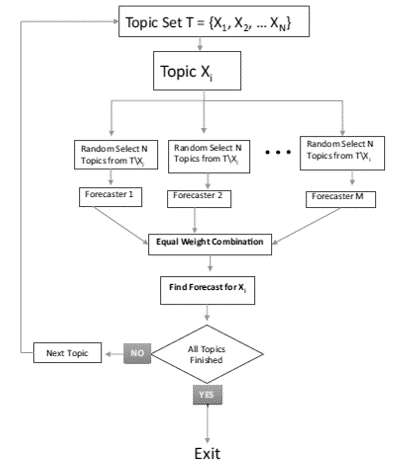
\includegraphics[width=0.5\linewidth]{01.Chapters/03.RelatedWorks/ensemble-forecasting-framework}
	\caption{Ensemble forecaster framework \cite{hurtado2016topic}.}
	\label{fig:ensemble-forecasting-framework}
\end{figure}





\section{Final Remarks}


